The data warehouse has been built with a particular structure, suited for both storing and processing the huge amount of data needed, as well as dealing efficiently with its high heterogeneity.

The various schemas created, as well as how they contribute to processing and exposing all the information, will be described in this chapter.
A final section will elaborate on a particular type of tables, which plays a very important role in the Data Warehouse.

\section{Schemas}
    The data warehouse contains several schemas, each one serving a specific purpose.

Two schemas, called \textit{Source} and \textit{Staging}, are used for loading the data, while a different one, called \textit{Data Mart}, contains the final data.

The first two schemas behave differently from the latter, since their purpose is to process the content of each \texttt{csv} file when inserting new data into the Data Warehouse.
These tables are emptied each time a different file is processed.

Several additional schemas, are also present in the data warehouse, but they have a less important role.

\subsection{Source}
    The \textit{Source} schema, named \texttt{src}, is where Databricks directly loads the \texttt{csv} data at the end of the ETL process.
    
    It contains a table for each data stream downloaded by Databricks.
    The structure of these tables is identical to the \texttt{csv} structure.
    All fields are of type \texttt{VARCHAR}, since all values loaded from \texttt{csv} are by default interpreted as strings.
    
    Each table in this schema has associated a view.
    These views are used to cast the data to their correct types as well as rename the fields into a standardized format.
        
\subsection{Staging}
    The \textit{Staging} schema, called \texttt{stg}, loads the data from the \texttt{stg} schema views and performs some more operations on them.
    
    The number of tables in this schema is much lower than the one in the \texttt{src} schema.
    This is because the data in this schema are aggregated together.
    
    \paragraph{Example}
        Let us take for example weather data.
        Information about weather come from several providers.
        Each one has different information: some providers may contain data about temperature and humidity, while others may have information about gas or power demand\footnote{
            These information are correlated.
            For example, on a cold day there is more need for heating and, as a consequence, a higher gas demand.
        }.
        In other cases, for example, a provider may be related to a single zone (e.g., energy consumption in Austria), so multiple providers are needed to get the whole European picture.\\
    
    In all these cases, it is necessary to group together data from different providers, since the information they provide are strictly correlated.
    
    This aggregation is done in this schema by apposite procedures.
    These procedures read data from the views present in the \texttt{src} schema.

\subsection{Data Mart}
    The \textit{Data Mart} schema, called \texttt{dm}, contains the first layer of data to be consulted by users.
    
    Data are loaded into this schema from the \textit{staging} stables.
    
    Tables in this schema are meant to be consulted by end-users for their daily needs.
    Information contained in this schema are both up-to-date and complete (i.e., each table contains data related to several years back and there are no missing values).
    
\subsection{DBO}
    The \texttt{dbo} schema contains remappings, which are used to normalize some data.
    
    Remappings will be described in section \ref{section:dwh:remappings}.

\subsection{Configuration}
    An interesting schema is the one called \texttt{configuration}, which contains some parameters which influence the ETL process executed by Databricks.
    
    Amongst all the parameters, two are of particular interest: the download time range, as well as retry information, in case of download failure.
    Table \ref{tab:dwh:configuration} is an example of configuration parameters stored in this schema.
    
    \begin{table}
        \centering
        \begin{tabular}{|c c|c c|c c|}
            \toprule
             Provider   & Stream      & From       & To   & Retries & Retry Delay \\
             \midrule
             Weather\_A & Temperature & 01/01/2017 & NULL & 3       & 10         \\
             Weather\_A & Humidity    & 01/01/2017 & NULL & 3       & 10         \\
             Weather\_B & Temperature & 01/01/2019 & NULL & 2       & 15         \\
             Weather\_B & Pressure    & 01/01/2018 & NULL & 5       & 5         \\
             \bottomrule
        \end{tabular}
        \caption{Some configuration parameters.}
        \label{tab:dwh:configuration}
    \end{table}
    
    \paragraph{Download time range}
        These information are used to specify when to stop when downloading data from a given provider.
        
        This parameter has two uses: first of all, in case the provider has more historical information than what needed, it limits the amount of data recovered.
        This not only reduces history download time, but also prevents too much unneeded data from being loaded into the data warehouse.
        In the opposite case, this parameter is also needed not to attempt to download historical data from a provider if we know it is not available.
        This prevents the downloader from encountering errors caused by non-existent files.
        
        A \texttt{NULL} value specifies that there is no time range limit.
    
    \paragraph{Retries}
        The downloaders have been programmed to attempt again to download data in case the provider timeouts.
        
        These parameters specify both how many attempts to perform, as well as the required delay between each attempt.
        
        Given the different importance and update frequency of the different providers, these values differ depending on which data is being downloaded.
    
    \paragraph{Remarks}
        It is important to notice that these parameters are not specified for each provider, but for each data stream.
        
        This decision has been made considering two factors.
        
        First of all, sometimes data from a single provider is recovered from multiple sources (e.g. different websites belonging to the same organization).
        Each source can present a different level of availability.
        
        Secondly, some data streams are more important than others.
        It is reasonable to spend more effort downloading this kind of data if they happen to be unavailable, otherwise some critical processes may stop working.

\subsection{Other Schemas}
    The Data Warehouse contains also other schemas, which play, however, a less important role in the data processing procedures.
    
    For example, the schema \texttt{trd} (\textit{Trading}) contains some views explicitly requested by the trading team.
    These views are just a simple manipulation of the data stored in the \textit{Data Mart} schema.
    Their purpose is exposing some data in a particular format, which is required by some tools used by the trading department.
    

    
\section{Remappings} \label{section:dwh:remappings}
    Some information can be expressed in different ways.

For example, the same hour can have different values depending on the timezone used.
Some providers also count hours from 0 to 23, while others use the most common 1-24 notation.

When dealing with this kind of data, it is important to choose a consistent and uniform way of these information.

This action is done through additional tables, used to remap the original data to the uniform notation used.

\subsection{Logic vs Materialized Remappings}
    Remappings can be either logical or materialized.

The former are created by joining any table with a remapping table, producing the results in the query output.
In the latter case, on the other hand, the results are physically stored on the data warehouse and do not require any join operation.

Let's now analyze the advantages and disadvantages of each remapping technique.

\subsubsection{Query performance}
    The type of remapping chosen can directly influence the performance of a query.

    \paragraph{Logical remappings}
        Logical remappings require to join each value of a given table with the remapping.
        This operation is applied to a large amount queries used by Axpo, since they require some information in a specific notation.
        
        The cost of the join is however low, since these remapping tables are usually very small, ranging from tens to a couple hundred rows.
        As such a single join can be computed very quickly, but it can become a problem if these operations need to be applied for almost each query.
        
    \paragraph{Materialized remappings}
        Materialized remappings require no additional overhead, since the remapped information are physically stored along the other data.
        
        This choice is ideal for values which are always used in their remapped notation.
        For example, each provider uses its own hour notation, while all Axpo tools use a standard numeric notation ranging from 1 to 25.
        
        Instead of having to perform a join for \textunderscore{every} query, it is more efficient to memorized this value directly into the table, removing the join overhead.
    
    
\subsubsection{Query complexity}
    Queries become more complex since they require join operations with additional tables.
    This scenario is even more complex when multiple remappings are needed for the same table.
    
    \paragraph{Logical remappings}
        For local remappings, each remapping needed results in a join operation.
        
        Sometimes, multiple columns referring to the same type of information need to be remapped.
        This leads to a more complex query, in which it is necessary to remember the name of each remap in order to avoid confusion.
        
        \begin{figure}
            \centering
            \begin{subfigure}{\textwidth}
                \centering
                \fbox{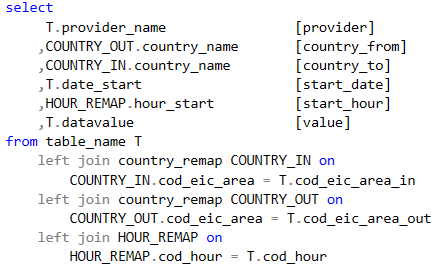
\includegraphics[width=.5\textwidth]{res/dwh/remap_logical.png}}
                \subcaption{Logical}
                \label{fig:dwh:remapping:complexity:logical}
            \end{subfigure}
            
            \begin{subfigure}{\textwidth}
                \centering
                \fbox{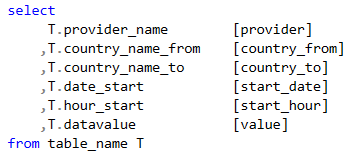
\includegraphics[width=.4\textwidth]{res/dwh/remap_materialized.png}}
                \subcaption{Materialized}
                \label{fig:dwh:remapping:complexity:materialized}
            \end{subfigure}
            
            \caption{Query complexity for different remappings. Both queries produce the same output.}
            \label{fig:dwh:remapping:complexity}
        \end{figure}
        
        As an example, the query shown in Figure \ref{fig:dwh:remapping:complexity:logical} represents a query using logical remappings.
        As we can see, multiple join operations are needed, making the query harder to read.
        
    \paragraph{Materialized remappings}
        Materialized remappings do not need any join operation, since the data is directly present in the table.
        As a consequence, queries are both easier to write and to read.
    
        The query shown in Figure \ref{fig:dwh:remapping:complexity:materialized} represents the same query as above, but uses materialized remappings.
        The query is certainly easier to read and to understand, and the possibility of making errors is minimized.

\subsubsection{Data insertion}
    When a new row is inserted additional operations have to be performed depending on the remapping type.
    
    \paragraph{Logical remappings}
        Logical remappings are more convenient during insertion, since they do not require any additional operation on the values inserted.
        
        The only check needed is that each value to be remapped is present in the remapping table.
        
        Otherwise an alert must be raised and an appropriate remapping has to be created.
    
    \paragraph{Materialized remappings}
        In case of materialized remappings, it is necessary to compute each remapping prior to the insertion operation.
        
        In case of missing values, there are two possibilities: either the row is not inserted or it is inserted with a temporary remapped value of \texttt{NULL}.
        In both cases an alert must be raised.

\subsubsection{Remapping changes}
    Remapping tables can be changed if errors are detected.
    Depending on the remapping type used for a specific values, different scenarios may occur.

    \paragraph{Logical remappings}
        Logical remappings handle changes to remapping tables very efficiently.
        
        Since the remapped value is computed at query time, no additional operation are needed on the table.
        
    \paragraph{Materialized remappings}
        Materialized remappings need to be updated each time the remapping table is modified.
        
        All remapped values are computed again by an apposite procedure (the same used during insertion).
        In case of incomplete remappings (e.g., a value from the remapping table has been removed), an alert must be raised.

\subsection{Examples}
    In this section, I will provide a few examples of the remappings created by Reply, to give a more hands-on idea of the notations used by different providers, as well as how they have been normalized.
    
Since I was constantly analyzing the Data Warehouse, I often noticed several small problems with remappings, such as wrong associations or missing values.
Each time I noticed a problem, I analyzed the cause and told Reply how to fix the issue.

In other cases, I directly asked Reply to remap additional data, which could be used to improve query performance or to simplify existing queries.

\subsubsection{Hours}
    The energy market presents different problems related to hour handling.
We will see them in detail, along with how they have been remapped.

\paragraph{Notation}
    The most apparent issue is the lack of a standard notation amongst all providers.
    
    \begin{table}
        \centering
        \begin{tabular}{|r|c|}
            \toprule
            Provider        & Hour format   \\
            \midrule
            EU Market 	    & 7             \\
            EU Market 	    & Hour 7        \\
            EU Market 	    & Volume H07    \\
            IT Market       & 7             \\
            EU Transfer     & 06            \\
            IT Transfer     & 06            \\
            IT Transfer     & 6             \\
            IT Transfer     & H07           \\
            \bottomrule
        \end{tabular}
        \caption{Different notations for the same hour (7 am).}
        \label{tab:dwh:remapping:hour:notation:7}
    \end{table}
    
    Table \ref{tab:dwh:remapping:hour:notation:7} shows an example of how the same hour is referred to by different providers.
    
    These different notations cause many problems during queries, since the same value has different meanings depending on the provider.
    
    As such, it is necessary to devise a solution to normalize all the hours into a single notation, independently of the provider.
    
\paragraph{Daylight Saving Time} \label{section:dwh:dst}
    One of the problems most commonly encountered is caused by Daylight Saving Time (DST).
    
    On the last Sunday of March, time is shifted one hour forward at 2am while, on the last Sunday of October, time is shifted one hour back at 3am.
    
    As a consequence, in March we have a day with 23 hours, since the hour between 2 and 3am is skipped, while in October we have a day with 25 hours, since the hour between 2 and 3am is repeated twice.
    
    The main problem is that each provider handles these hours in their own way, using their own notation.
    As a consequence, the same value may have different meanings depending on the provider.
    
    Some providers, for example, start numbering the hours from 0, while others start from 1.
    In this case, it becomes clear that a value of \texttt{1} can indicate either \texttt{0am} or \texttt{1am}.
    
    An additional problem is also given by the lack of a standard notation for expressing the hours between 2am and 3am on the last Sunday of October, which are repeated twice.
    The second repetition needs however to be distinguished with a different notation.
    Table \ref{tab:dwh:remapping:hour:notation:3} shows how these hours are referred to by different providers.
    
    \begin{table}
        \centering
        \begin{tabular}{|c|c c c c c|}
            \toprule
            Provider    & 0am        & 1am        & 2am         & 2am (2)     & 3am        \\
            \midrule
            Forecasts	& 0          & 1          & 2           & 3           & 4          \\
            Weather	    & 0          & 1          & 2A          & 2B          & 3          \\
            % \midrule
            Market A	& 1          & 2          & 3           & 4           & 5          \\
            Market B	& 1          & 2          & 3           & 4           & 5          \\
            Market B	& Volume H01 & Volume H02 & Volume H03A & Volume H03B & Volume H04 \\
            Market C	& 1          & 2          & 3           & 3B          & 4          \\
            Market C	& Hour 1     & Hour 2     & Hour 3A     & Hour 3B     & Hour 4     \\
            Market C	& Volume H01 & Volume H02 & Volume H03A & Volume H03B & Volume H04 \\
            Market D	& 1          & 2          & 3           & 4           & 5          \\
            % \midrule
            Transfer A  & 1          & 2          & 3           & 4           & 5          \\
            Transfer A  & ORA01      & ORA02      & ORA03       & ORA04       & ORA05      \\
            Transfer B  & 0          & 1          & 2           & 3           & 4          \\
            Transfer C  & 0          & 1          & 2A          & 2B          & 3          \\
            \midrule
            Remapped to & 1          & 2          & 3           & 4           & 5          \\
            \bottomrule
        \end{tabular}
        \caption{
            Different hour notations during DST changes (on last Sunday of October).
            The last row specifies the remapped value for all occurrences.
        }
        \label{tab:dwh:remapping:hour:notation:3}
    \end{table}

\paragraph{Gas Day} \label{section:dwh:gas_day}
    Gas providers handle dates in a different way, using a particular notation called \textit{Gas Day}.
    Gas days start at 6am and end at 6am of the next day.
    
    Differently from standard dates, there are no DST changes, which means that each day across the whole year has 24 hours.
    During DST, each day is as a consequence shifted by an hour (gas days start and end a 7am).
    
    As a consequence, each file retrieved from gas providers contains data about to two different days: the hours 6-24 are related to a given day, while the remaining (24-6), are related to the following one.
    
\paragraph{Timezones}
    Some websites provide dates in local time, which means that these dates must take into account GMT.
    
    Additional problems are presented by DST changes.
    For example, DST changes in the UK occur between 1am and 2am (local time), which, taking into account the GMT difference, is the same time as 2-3am (the moment DST changes in Italy).
    
    This means that the same hour not only changes meaning depending on the provider, since each one has its own notation, but also on the geographical zone.
        
\paragraph{Solution}
    The solution is to create a table which specifies how to remap each hour into their actual value.
    
    Considering that most queries will need this kind of data, as well as the fact that remaps are likely not to change for existing data, it has been chosen to materialize the remapped hours directly into the tables.
    
    In this way, users will expect faster computational times, as well as simpler queries.
    
\subsubsection{Countries}
    Countries can be referred to in different ways.
As such it is necessary to normalize these information.

\paragraph{Problems}
    Providers refer to countries in two different granularities.
    
    The most generic information indicates the country itself, while the most detailed specifies a smaller zone, which belongs to a specific country.
    These zones are specific to the energy sector and divide a country based both on geographical and energetic factors.
    
    Not all countries are divided in zones.

    \subpar{Countries}
        Most providers use the same notation for expressing countries.
        
        However there are a few exceptions.
        For example, some providers spell countries in a different way or using a different case.
        Some other providers refer to countries using a two-character ISO notation\footnote{
            Standard notation commonly used worldwide.
            For example, Italy is abbreviated `IT' and United States `US'.\\
            For a comprehensive list of country codes, see \cite{bib:country_codes}.
        }.
        
        As such, the data needs to be remapped into a common notation, to preserve consistency amongst all data.
        This remapping is done through an apposite table, such as the one shown in table \ref{tab:dwh:remapping:country}.
        
        \begin{table}
            \centering
            \begin{tabular}{|c|c|}
                \toprule
                Original            & Remapped      \\
                \midrule
                Belgian	            & Belgium       \\
                Belgium	            & Belgium       \\
                \midrule
                Germany             & Germany       \\
                germany\_luxembourg	& Germany       \\
                Germany/Luxembourg	& Germany       \\
                \midrule
                netherlands	        & Netherland    \\
                Netherland	        & Netherland    \\
                \midrule
                PT	                & Portugal      \\
                Portugal	        & Portugal      \\
                \bottomrule
            \end{tabular}
            \caption{Country remappings.}
            \label{tab:dwh:remapping:country}
        \end{table}
        
    \subpar{Country zones}
        Country zones are either referred to directly or by using a particular notation known as \texttt{EIC}\footnote{
            \textit{Energy Identification Codes}.
            These coding scheme is used across Europe to facilitate cross-border exchanges and to efficiently and reliably identify different objects and parties relating to the Internal Energy Market and its operations \cite{bib:enstoe:eic}.
        }.
        
        In the first case no normalization operations are needed, while in the second, it is necessary to remap these codes to both a normalized version of the zone name as well as to the country it belongs to.
        
        \begin{table}
            \centering
            \begin{tabular}{|c|l c|}
                \toprule
                EIC                 & Zone                  & Country   \\
                \midrule
                10YIT-GRTN-----B	& Italy	                & Italy     \\
                10Y1001A1001A73I	& Italy\_NORD           & Italy     \\
                % 10Y1001A1001A70O	& Italy\_CNOR           & Italy     \\
                % 10Y1001A1001A71M	& Italy\_CSUD           & Italy     \\
                10Y1001A1001A788	& Italy\_SUD            & Italy     \\
                10Y1001A1001A75E	& Italy\_SICI	        & Italy     \\
                10Y1001A1001A83F	& Germany               & Germany   \\
                10YDE-ENBW-----N	& Germany\_TransnetBW   & Germany   \\
                \bottomrule
            \end{tabular}
            \caption{EIC codes and remapped values.}
            \label{tab:dwh:remapping:country_zone}
        \end{table}
        
        Table \ref{tab:dwh:remapping:country_zone} shows an example of \texttt{EIC} codes, as well as their remapped values.
        
\paragraph{Solution}
    Two additional tables have been created, containing remapping information for both countries and zones.
    
    These tables are similar to tables \ref{tab:dwh:remapping:country} and \ref{tab:dwh:remapping:country_zone}.
    
    Since not all queries require this kind of data, the remapping are performed only at logical level.
    As such, new queries require to perform join operation with the remap tables.
    
    On the other hand, several views created for specific departments already perform these join operations, simplifying user interaction.
    
    The size of these tables are small (less than 100 rows), so the performance impact is negligible.
    
\subsubsection{Bidding Operation Types}
    Some providers use different notations when referring to bidding operations type.

Market bids can refer either to purchases of sales.
Each provider represents this information in its own format.

As such, it is necessary to create a remapping table to normalize this notation.
The table needs to know both the original format as well as the provider, since different providers may use the same value for different things.

\begin{table}
    \centering
    \begin{tabular}{|c|c|c|}
        \toprule
        Provider    & Original  & Remapped  \\
        \midrule
        Provider\_A & P         & Purchase  \\
        Provider\_A & S         & Sell      \\
        Provider\_B & Purchase  & Purchase  \\
        Provider\_B & Sell      & Sell      \\
        Provider\_C & BID       & Purchase  \\
        Provider\_C & OFF       & Sell      \\
        Provider\_D & C         & Purchase  \\
        Provider\_D & V         & Sell      \\
        \bottomrule
    \end{tabular}
    \caption{Bidding operation type remappings.}
    \label{tab:dwh:remapping:op_type}
\end{table}

The resulting table is similar to table \ref{tab:dwh:remapping:op_type}.

The table hasn't been materialized given its very small size (less than 10 elements).


% \subsubsection{Granularity / Estimation Period}
%     Most of the data downloaded by the ETL process have a column indicating its granularity or to how which day it refers to (in the case of forecasts).

\begin{table}
    \centering
    \begin{tabular}{|c|c|}
        \toprule
        Original & Remapped \\
        \midrule
        15M& \\
        60M& \\
        \bottomrule
    \end{tabular}
    \caption{Granularity remappings}
    \label{tab:dwh:remapping:granularity}
\end{table}

\begin{table}
    \centering
    \begin{tabular}{|c|c|}
        \toprule
        Original & Remapped \\
        \midrule
        D& \\
        D+1& \\
        D+7& \\
        M& \\
        \bottomrule
    \end{tabular}
    \caption{Granularity remappings}
    \label{tab:dwh:remapping:granularity2}
\end{table}

Reply has chosen to use the notation reported in the first column of Table \ref{tab:dwh:remapping:granularity}.

